\section{Water-Quality Monitoring Results}
\label{sec:results-water}

The water-quality module raises a different question from the vibration module. Its decision rules
are fixed comparisons against limits, so the harder question is whether the readings that reach them
can be trusted. The results therefore separate three kinds of evidence, in the order of
Section~\ref{sec:meth-wq}: known-input experiments that test the decision logic and the operator
settings (Section~\ref{sec:res-wq-logic}), hardware experiments that characterise each physical sensor
(Section~\ref{sec:res-wq-physical}), and fault experiments that test whether an invalid or missing
signal is reported as unavailable (Section~\ref{sec:res-wq-validity}).

% ------------------------------------------------------------
\subsection{Known-Input Verification and Configuration}
\label{sec:res-wq-logic}

This subsection asks whether the module turns a given reading into the correct condition and keeps
the operator's settings, independently of how good the reading is. It reports the simulation
experiment W-SW, including the earlier firmware stage whose failure led to a design change, and the
hardware experiment W-CONF on the settings form. Together they test the decision logic behind FR-W01
to FR-W03 and the persistence required by FR-S03.

\paragraph{Simulation experiment W-SW: decision logic under known inputs.}
The firmware's test mode replaced each sensor reading with a scripted value, marked every such
reading as simulated in the status data, and compared the resulting condition with an expected
condition written into the firmware. Because it ran on the ESP32 itself, it exercised the deployed
code; because the inputs were synthetic, it verifies the decision logic and not the sensors. All 45
steps passed, with no failure (Table~\ref{tab:res-wsw}). The four conversion steps turned fixed
voltages into pH 7.00, 4.00, 7.20 and 7.80 through a fixed calibration, each matching its expected
value to 0.01. The pH steps placed the input at 7.19, 7.20 and 7.21 and at 7.79, 7.80 and 7.81
(Figure~\ref{fig:res-ph-logic}a): 7.19 and 7.81 were classified as WARNING and the four values
between as CAUTION, which shows that both limits are inclusive and that the classification resolves
a change of 0.01 at each limit. The temperature and turbidity steps did the same for the preferred
range and the clarity threshold.

\begin{table}[H]
\centering\begingroup\methodtabset
\caption{Known-input checks of the final water-quality firmware (simulation experiment W-SW). Each
step compared the reported condition with an expected condition written into the firmware.}
\label{tab:res-wsw}
\begin{tabularx}{\linewidth}{|Q{2.4cm}|Q{1.3cm}|Z|}
\hline
\textbf{Scenario} & \textbf{Passed} & \textbf{Conditions exercised} \\
\hline
pH conversion & 4 of 4 & Voltage to pH through a fixed calibration, to 0.01 \\ \hline
pH & 17 of 17 & OK, CAUTION and WARNING on both sides of each limit; short spike; invalid input; recovery \\ \hline
Temperature & 12 of 12 & In, below and above the preferred range; unavailable; recovery \\ \hline
Turbidity & 12 of 12 & CLEAR and CLOUDIER about the clarity threshold; unavailable; recovery \\ \hline
\end{tabularx}
\endgroup
\end{table}

The status data recorded between the checked steps show the 30~s hold working as designed
(Figure~\ref{fig:res-ph-logic}b). A new zone became the reported status only after it had persisted
for 30~s, and in the ten changes between valid zones the measured delay was 29.3 to 30.7~s, within the
1~s spacing of the status polls. While a WARNING zone awaited confirmation, the possible-breach flag
was raised, so the operator is told that a limit has been crossed before it is confirmed. The 4~s spike
to pH 7.9 raised that flag and left the reported status at OK, which is the purpose of the hold: a
brief excursion is shown as a possible breach, not as a confirmed WARNING.

\begin{figure}[H]
\centering
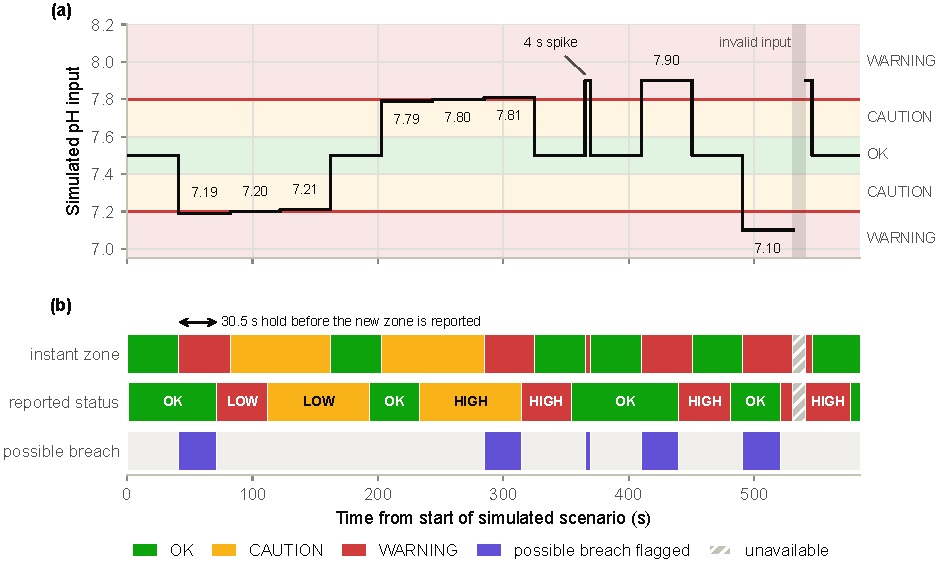
\includegraphics[width=\linewidth]{figures/fig5_6_ph_logic.pdf}
\caption{pH decision logic under the firmware's test mode (simulation experiment W-SW, final stage 5
firmware, status polled once per second). (a)~Scripted pH input, with the 7.2 and 7.8 limits, the
CAUTION margins and the values of the boundary steps. (b)~Zone of the current reading, status
reported after the 30~s hold, and the possible-breach flag. Labels in the reported row give the
direction (LOW or HIGH) of a CAUTION or WARNING status.}
\label{fig:res-ph-logic}
\end{figure}

The same experiment run on the earlier stage 4 firmware exposed a defect that its checks did not.
Every stage 4 step passed, but the status data showed what happened after the invalid input
(Figure~\ref{fig:res-ph-recovery}). When the input returned at pH 7.5, the zone of the current reading
was OK at once, yet the reported status went back to the WARNING~LOW held before the invalid input
and stayed there for a further 30~s. The firmware had restored a status that no longer described the
water, so an operator would have been shown a pH warning that did not apply. The stage 5 firmware
adopts the first valid zone after an invalid input directly instead of restoring the earlier status.
In its run the input returned at pH 7.9, and WARNING~HIGH was reported at once rather than the earlier
WARNING~LOW; the later change back to OK then followed the normal 30~s hold. The two scripts returned
at different values, so the exact stage 4 condition was not repeated, but the stage 5 run shows the
property that stage 4 lacked: the status after an invalid input is taken from the new reading. The
defect was found because the experiment recorded the full status stream and not only the pass or fail
of each step, a lesson that applies to any test built on discrete checks.

\begin{figure}[H]
\centering
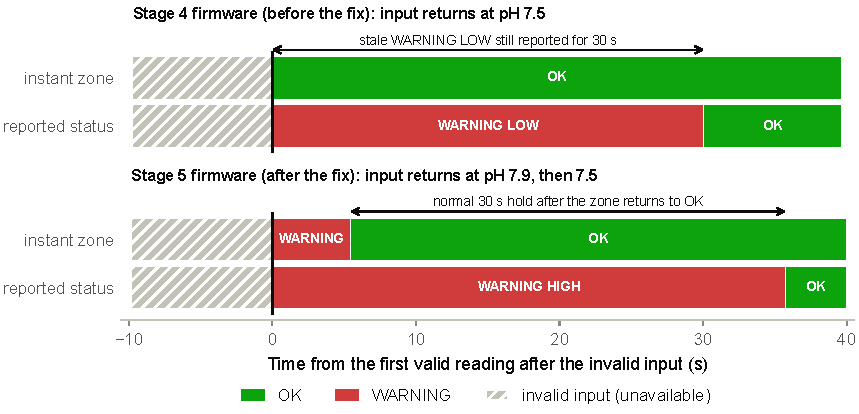
\includegraphics[width=\linewidth]{figures/fig5_7_ph_recovery.pdf}
\caption{Recovery after an invalid pH input in the stage 4 firmware, before the fix, and in the final
stage 5 firmware (simulation experiment W-SW). Time zero is the first valid reading after the invalid
input. Hatched: invalid input, reported as unavailable.}
\label{fig:res-ph-recovery}
\end{figure}

\paragraph{Hardware experiment W-CONF: operator settings.}
The settings form was tested on the hardware against five outcomes written in advance, and three were
met in full (Table~\ref{tab:res-wconf}). Both invalid entries were refused with a message that named
the rule, and nothing was saved. A valid entry was saved and an unchanged resubmission saved nothing.
The status data reported no restored settings in all 60 polls after the first start-up and restored
settings in all 30 polls after the restart, and the restored-settings lines appeared in all 18 later
start-ups recorded with this firmware.

\begin{table}[H]
\centering\begingroup\methodtabset
\caption{Operator settings on the hardware (experiment W-CONF). Messages are quoted from the board's
log.}
\label{tab:res-wconf}
\begin{tabularx}{\linewidth}{|Q{3.3cm}|Z|Q{2.8cm}|}
\hline
\textbf{Check} & \textbf{Result} & \textbf{Criterion} \\
\hline
Preferred pH 8.5 & Refused: ``Preferred pH must be between 7.2 and 7.8. The pH operating limits cannot be changed here.'' & Met \\ \hline
Temperature minimum above maximum & Refused: ``Temperature minimum must be below the maximum.'' & Met \\ \hline
Valid save: 20.0 to 30.0~$^\circ$C, pH 7.50 & Both values saved; condition ABOVE RANGE & Partly met: ``in range'' not observed \\ \hline
Unchanged resubmission & ``No changes.''; nothing saved & Met \\ \hline
Restart & Values restored in 18 of 18 later start-ups; condition ABOVE RANGE & Partly met: ``in range'' not observed \\ \hline
\end{tabularx}
\endgroup
\end{table}

The two partly met outcomes share one cause, and it lies outside the settings logic. The test sheet
expected the temperature condition to read ``in range'' once the 20 to 30~$^\circ$C range was saved,
on the condition that the room was within it. The probe read a mean of 32.1~$^\circ$C after the save
and 30.6~$^\circ$C after the restart, so ABOVE RANGE was the correct condition for those readings and
the ``in range'' outcome could not occur. The cause of the warm readings was not identified; the same
probe read 21.5~$^\circ$C in room air in a later experiment (Section~\ref{sec:res-wq-physical}). The
settings logic is therefore verified, but the hardware run did not observe the temperature condition
inside the saved range.

Taken together, the known-input and settings experiments establish, W-SW in simulation and W-CONF on
hardware, that the module applies the fixed pH limits independently of the preferred value, resolves
a 0.01 change at each limit, holds a new zone for 30~s while flagging a possible breach, takes its
status from the new reading after an invalid input, and keeps the operator's settings across restarts.
They do not establish that any reading is accurate, which is the subject of
Section~\ref{sec:res-wq-physical}.
